\section{Approach}
\label{sect:approach}
In this section, we describe the design and implementation of our system. 
We first present the overview of our design and then describe the each component in detail.

\subsection{Overview}

\begin{figure}[htb]
\centering
\includegraphics[width=0.5\textwidth]{arch}
\caption{The architecture of our system.}
\label{fig:architecture}
\end{figure}

\reffig{architecture} shows the high-level architecture of our system.
Users could get the statistics of the network and configure QoS requirements for the services they are using via a Web portal. Users specify the mininum rate, recommended rate and priority they want for each application. 

When the first packet of a flow arrives at the switch, a
copy of this packet is forwarded to the controller. The switch
continues to perform default forwarding of the traffic flows until
application identification has been performed, essentially
“lazily” implementing QoS only once application classification
is complete. The controller determines which classifier
should classify the application type for the flow. Each application
type is associated with a different queue, each of
which is shaped according to the traffic shaping policy for the application.

\subsection{Configuration Module}
In the configuration file, users only need to configure 3 parameters for a services. The following figure is part of a configuration file.
The minimum rate parameter specifies the minimum bandwidth the service requires.The recommended rate parameter specifies the desired bandwidth for the service.
The priority parameter specifies the users' prefenrece for the service.
For example, in the figure, the minimum rate for video is 1.5M and the recommended rate for vidoe is 7M. The priority for video, which is 10, is much higher than other types of services. So our SDN controller will try to first satisfy the QoS requirements for the video services in the network.

User define configuration in YAML format
\subsection{Flow classfier module}
The flow classifier maintains a lookup table where the key is a flow’s five-tuple (e.g., source IP address, destination IP address, protocol, source port, and destination port). When a
sender initiates a new flow, the switch sends a copy of the first packet of the flow to the controller. The flow classifier then checks whether the flow’s tuple correspond to an entry in this lookup table. The lookup then returns the type of application, such as video, VoIP, P2P, gaming, or web.

As traffic classification is not the focus of our project, in our implementation, we use static flow classifer to classfity the traffic.

It is very easy to extend our traffic classfication module to be more fine-grained and flexible. For example, we can easily integrate other approaches, such as DNS-based classifier~\cite{Seddiki_HotSDN14}, to our module. Or we can use the nmeta project~\cite{nmeta} as our traffic classification module.

\subsection{Traffic monitor module}



\begin{itemize}
\item Flow statistics
\item Port statistics
\end{itemize}
\subsection{Control Module}
On a high level, our control module tries to satisfy a maximum number of QoS requirements with the limited bandwidth.
Each type of service has been configured by the user with a priority. We assign a weight to the service based on the actual bandwidth it will get. For example, the weight of a service is 0.6 if the minimum rate bandwidth is achieved. The weight is 1.0 if the recommended rate bandwidth is achieved.
Our algorithm allocates bandwidth to different services to get the maximum value of $$\sum_{i=1}^{n} Weight_i*Prioriy_i $$ under the condition that
$$\sum_{i=1}^{n} Bandwidth_i <= C $$. C is the total bandwidth of the network.


\subsubsection{Dynamic queue assignment algorithm}

\begin{figure}[htb]
\centering
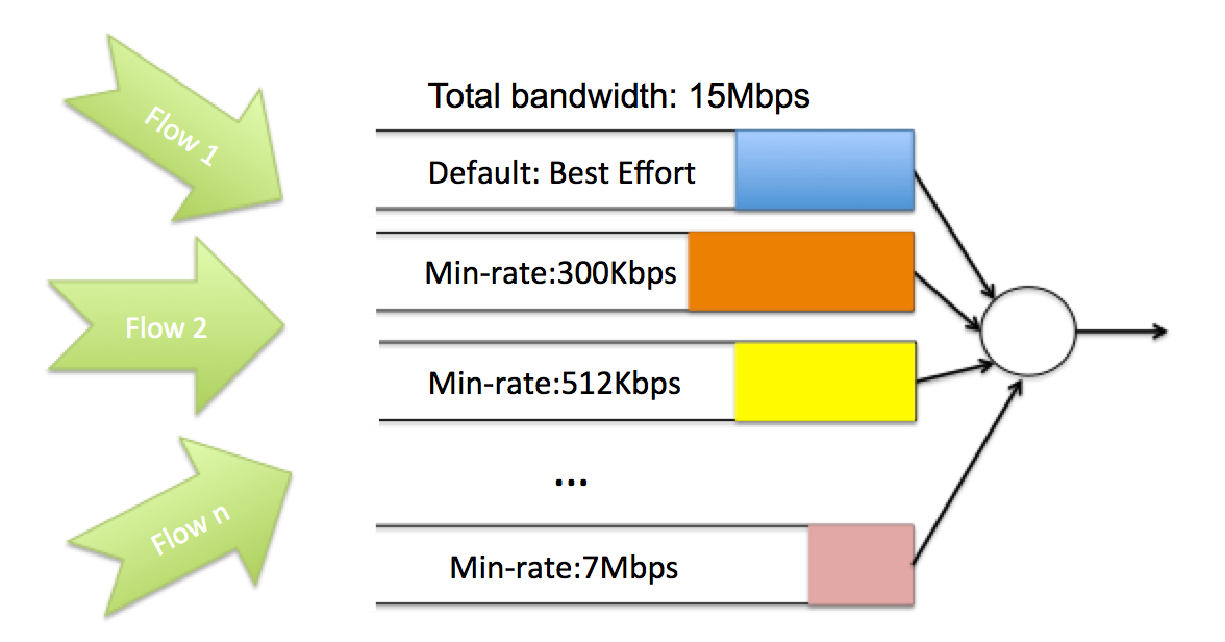
\includegraphics[width=0.5\textwidth]{assign_queue}
\caption{}
\label{fig:assign_queue}
\end{figure}

\subsection{Web Portal Module}
This module is for user configuration and traffic statistics.


\subsection{Implementation}
Implementation is based on Ryu SDN controller~\cite{ryu} and OpenVSwitch.
